% !TEX root = thesis.tex
\chapter{はじめに}
\label{chap:preface}
\section{Web工学と機械学習}
近年Web工学の領域においては、広告の効率アップや文章の分析、検索エンジンの性能向上などが求められている。このため、ユーザの性格や行動の分析、ネットワーク構造の未来予測、文章の意味や感情の理解といった技術が必要とされている。
例えば、Web上で物を販売しているサイトにおいて、ユーザが購入しそうな商品を勧め、売り上げを増大させることを考える。ユーザが今まで見た商品、購入した商品を分析して、ユーザの求めている商品のジャンルを知ったり、Webショッピングにおける性格を知ることが出来れば、ユーザが買いたい商品を先回りして、広告表示することが出来る。ユーザに対して、より購入してくれそうな広告を多く見せて、広告の効率をアップさせることで、サイトからの収益が上がることが期待できる。
Web工学では、Web上のデータを元に知識を学習し、次に得た知識を用いて予測や分類を行う、というアルゴリズムが必要になっている。例えば、ユーザ行動やソーシャルネットワーク構造の傾向を学習して、将来の動向を予測したり、ユーザに送られたメールの意味を理解できるようになって、迷惑メールとそうでないものを分類できるようになる、といった具合である。こういった知識学習のためには、機械学習(マシンラーニング)と呼ばれる手法が広く用いられている。
機械学習とは、対象となる知識を数学的なモデルで表し、より適切なモデルを求めて微修正を重ねることで、知識を洗練させていくアプローチである。使用する数学的なモデルの大筋は、経験を基にあらかじめ決めておく。ユーザ行動、リンク構造、メールの文章といった元データは、全て数値に変換されて、モデルに入力される。モデルは、入力データから予測や識別を実際に行いつつ、より良い結果が得られるように、モデル内の係数を調整していく。最終的に、多種多様なデータに対して、適切な予測や識別を行うことが出来る数学的モデルを得ることができるのである。

\section{深層学習の台頭}
機械学習における大きなポイントの1つに、元データをどのような数値データに変換するか、という問題がある。\\
変換された数値データのことを、 特徴量、あるいは素性(feature)と呼ぶ。機械学習は、「生データから素性への変換」「素性をモデルに入力」「モデルによる数値計算で、結果を出力」「結果がより正確になるよう、モデルを修正」というプロセスの繰り返しで成り立っている。このうち、「素性への変換」だけは、画像・文章・リンク構造といった、データの種類に依存している。いったん素性が数値の形で得られれば、残りのプロセスは、データの種類に依存せず、全て入力数値とモデルの関係だけで解決することができる。つまり、機械学習のプロセスは、データの種類に依存する素性変換と、汎用的に使えるモデル学習の部分に分かれているのである。\\
機械学習の性能を上げるためには、素性への変換部分を工夫する方法と、使用する数学的モデルを洗練する方法の2つがある。素性への変換部分の改良は、対象となるデータの種類に強く依存している。例えば、画像データを素性数値に変換する場合、単純なRGB画素データをそのまま使っても良いが、SIFT特徴量やSURF特徴量、フィッシャーベクトルなど、より画像の特徴を捉えた特徴量を用いることが定石となっている。音声データに対しては、時間領域や周波数領域の波形をそのまま用いても良いが、メル周波数ケプストラム係数と呼ばれる特徴量も用いられる。問題とデータ種別に応じて、利用する特徴量を工夫することにより、機械学習の識別精度や実行時間などの性能が向上することが知られていた。このとき、特徴量はそれぞれのデータの専門家による、謂わば職人芸によって作られていた。
2000年代半ばに、Deep Learningと呼ばれる一群の手法が台頭した。Deep Learningとは機械学習の手法の1つで、人間の脳の構造に類似した、多層ニューラルネットワーク構造をモデルに用いて、学習を行わせる方法である。Deep Learningは、画像認識や音声認識、化合物の生成予測といった分野で優れた性能を示し、注目を浴びるようになった。図\ref{c1_nikkei}は、多層ニューラルネットワークが人間の脳の思考回路である、神経細胞のつながりを模倣する様子を表している。(日経ビジネス2013年4月号より一部抜粋)\\
\begin{figure}[tbp]
 \begin{center}
  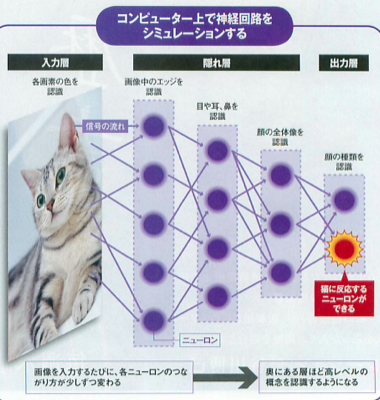
\includegraphics[width=80mm]{img/c1/nikkei}
 \end{center}
 \caption{ディープラーニングで画像を認識する流れ}
 \label{c1_nikkei}
\end{figure}
Deep Learningの特徴の一つとして、生の入力データから自動的に素性を作り、抽象表現を習得する働きがあると考えられている。例えば人間の顔画像データを学習させた場合、多層ニューラルネットワークを構成する複数のレイヤーのうち、入力に近い低レイヤーのニューロンは、画像のエッジ部分に対して強く反応し、出力に近い高レイヤーのニューロンでは、目口鼻、さらに顔全体など、より抽象度の高い要素に対して反応することがわかった。これは、見方を変えれば、低レイヤーでは中間表現(素性にあたる)を抽出しており、低レイヤーで得た素性を高レイヤーに入力することにより、より高レベルな抽象的概念に対しても優れた識別精度を実現している、と考えられる。どのような素性を使えば良い結果が出るのか、素性の抽出方法自体を同時に機械学習していることから、Deep LearningはRepresentation Learning(表現学習)とも呼ばれている。\\
GoogleのDeep Learning研究グループは2012年、Youtubeのビデオによる学習を長時間行わせることで、ニューラルネットワークの1つのニューロンが、猫の画像(\ref{c1_catdetection}、Googleの研究紹介記事より引用\footnote{\url{http://googleblog.blogspot.jp/2012/06/using-large-scale-brain-simulations-for.html}})を認識するようになったと発表し、大きな話題を呼んだ\cite{Le:2012:BHFBHFULSUL:00}。このYoutubeビデオ学習の間、「この画像は猫という名前のものである」「猫を認識できるよう学習を行いなさい」といった、認識ラベルの付け方における指針は一切学習器に与えられなかった(教師無し学習)。それにも関わらず、多層ニューラルネットワークは、自然と「この(我々の言葉でいう猫の)画像は覚えておくべきである」というように、何を認識すると学習効率が良いのか、何を素性とすれば学習がしやすいのか、という情報自体を学習することが出来た。また、同じ論文にて、この多層ニューラルネットワークが人間の顔を学習できることも示された(\ref{c1_facedetection}、\cite{Le:2012:BHFBHFULSUL:00}より引用)。\\
\begin{figure}[tbp]
 \begin{center}
  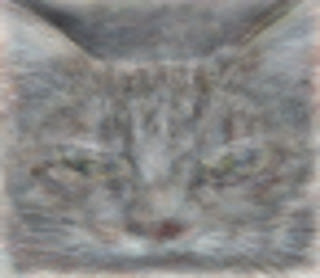
\includegraphics[width=50mm]{img/c1/cat_detection}
 \end{center}
 \caption{猫を認識するニューロン (教師無しYoutubeビデオより学習された。)}
 \label{c1_catdetection}
\end{figure}
\begin{figure}[tbp]
 \begin{center}
  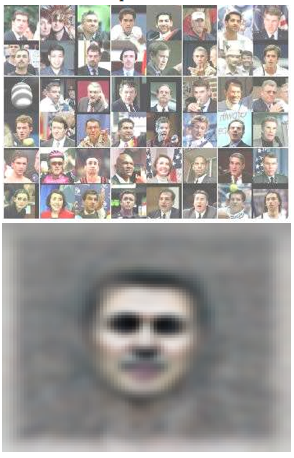
\includegraphics[width=50mm]{img/c1/google_face}
 \end{center}
 \caption{上 : 入力画像の中で、ニューロンが最も強く反応した48枚 下 : 計算上、最もニューロンが強く反応する画像}
 \label{c1_facedetection}
\end{figure}


\section{深層学習の課題と、研究の目的}
Deep Learningが高い識別性能を持つことがわかり、Deep Learningを身近な問題に適用して、良い成果を得たいという機運が高まっている。例えば、Web工学の分野では機械学習が大きな役割を果たしており、この学習プロセスにDeep Learningを組みこむことで、学習精度が向上したり、より多様な情報を扱えるようになる可能性がある。出来るだけ簡易に、Deep Learningを様々な問題に応用するための方法論が求められている。\\
しかし、Deep Learningは歴史の浅い発展途上の技術であり、どのアルゴリズムを定番とすれば良いのか、試行錯誤の段階にある。これは、各アルゴリズムの改良点が次々と見つかっていることに加え、学習性能が高くなる原理や、各アルゴリズムの得手不得手など、解明されていない部分が多いことが、主な原因である。アルゴリズムが開発途上で確定できていないため、公開されているライブラリも、現状では、開発用途や実験的なものが多くなってしまっている。実験的なライブラリでは、一部の種類のデータにのみ適用されることを想定して書いている場合があり、他の種類のデータを扱うためには、データ変換用のソースコードを記述しなければならないケースが多い。そもそも有力なアルゴリズムに対応する実装が公開されていない場合もあり、この場合、アルゴリズムの部分も含めて全ての実装を用意しなければならない。また、問題に応じて自らアルゴリズムの細部を調整しなければならない場合もある。例えば、学習の繰り返し回数(エポック数)や、どの種類のレイヤーを何回重ねるべきか(レイヤー構造)、1つのレイヤーに含まれる学習素子(ニューロン)の個数はどうするか、などである。これらはソースコードの作成者が経験的に手作業で調整しているケースが多く、標準と言える公開ライブラリが確立していない状況なので、Web工学など応用分野にDeep Learningを適用したいと考えても、プログラム開発に長い時間がかかってしまう。開発における大きな障壁となっている。\\
さらに、現在のDeep Learning技術では、他のアルゴリズムに比べて学習にかかる時間が長いことが多く、ハードウェア性能が低いマシンでは、アルゴリズムを実用的な時間で実行すること自体が容易ではない。実行時間の長さをカバーするため、GPUを用いて演算をスピードアップさせる手法が確立されつつあるが、特殊なプログラミングが要求され、開発における障壁の1つとなっている。また、ノートPCの大部分など、並列演算に利用可能なGPUを搭載していないPCを使っている場合には、ライブラリがGPUを利用しているために、却ってその実行が不可能になってしまうこともある。\par
以上に挙げた原因により、Deep Learning技術に関心を持っていても、まず実際の問題にDeep Learningを試行すること自体が困難であり、応用技術開発のハードルは更に高くなっている。特に、国内での研究開発は遅れており、早急なキャッチアップが必要である。\par
本研究では、このような現状を踏まえ、Deep Learning技術を実際の問題に応用するための方法論を確立すると共に、実装における障壁を出来る限り取り除くことを目指す。特にWeb工学における応用を目標とする。\\
2章では、従来のWeb工学における機械学習の応用方法と、Deep Learning出現以前に良く用いられていた、機械学習による識別器学習方法について、俯瞰する。3章では、Deep Learningを構成する個々のアルゴリズムについて、その原理と詳細を述べる。4章では、実際にDeep Learningアルゴリズムを利用する上で、どのように実装を進めれば、Deep Learningの特徴である高い学習性能を確実に利用できるのか、また、現実の問題を解決するときに重要となる、実行時間の短さ、実行プログラムの使いやすさ、アルゴリズムの調整・改良の容易さなどは、どのようにすれば確保できるのか、といったDeep Learningを使っていく上でのノウハウを記述する。\\
5章と6章では、4章までの内容を実際の問題に応用することで、その有用性を確かめる。5章では、Deep Learningのプログラムを、汎用的なベンチマークにかけることで、その性能を測定・比較する。6章では、ソーシャルメディア上のプロフィール画像を分類させるタスクに、Deep Learningを応用する。5章と6章の結果を受けて、7章ではDeep Learningを利用していく上でのベストプラクティスを提案する。
